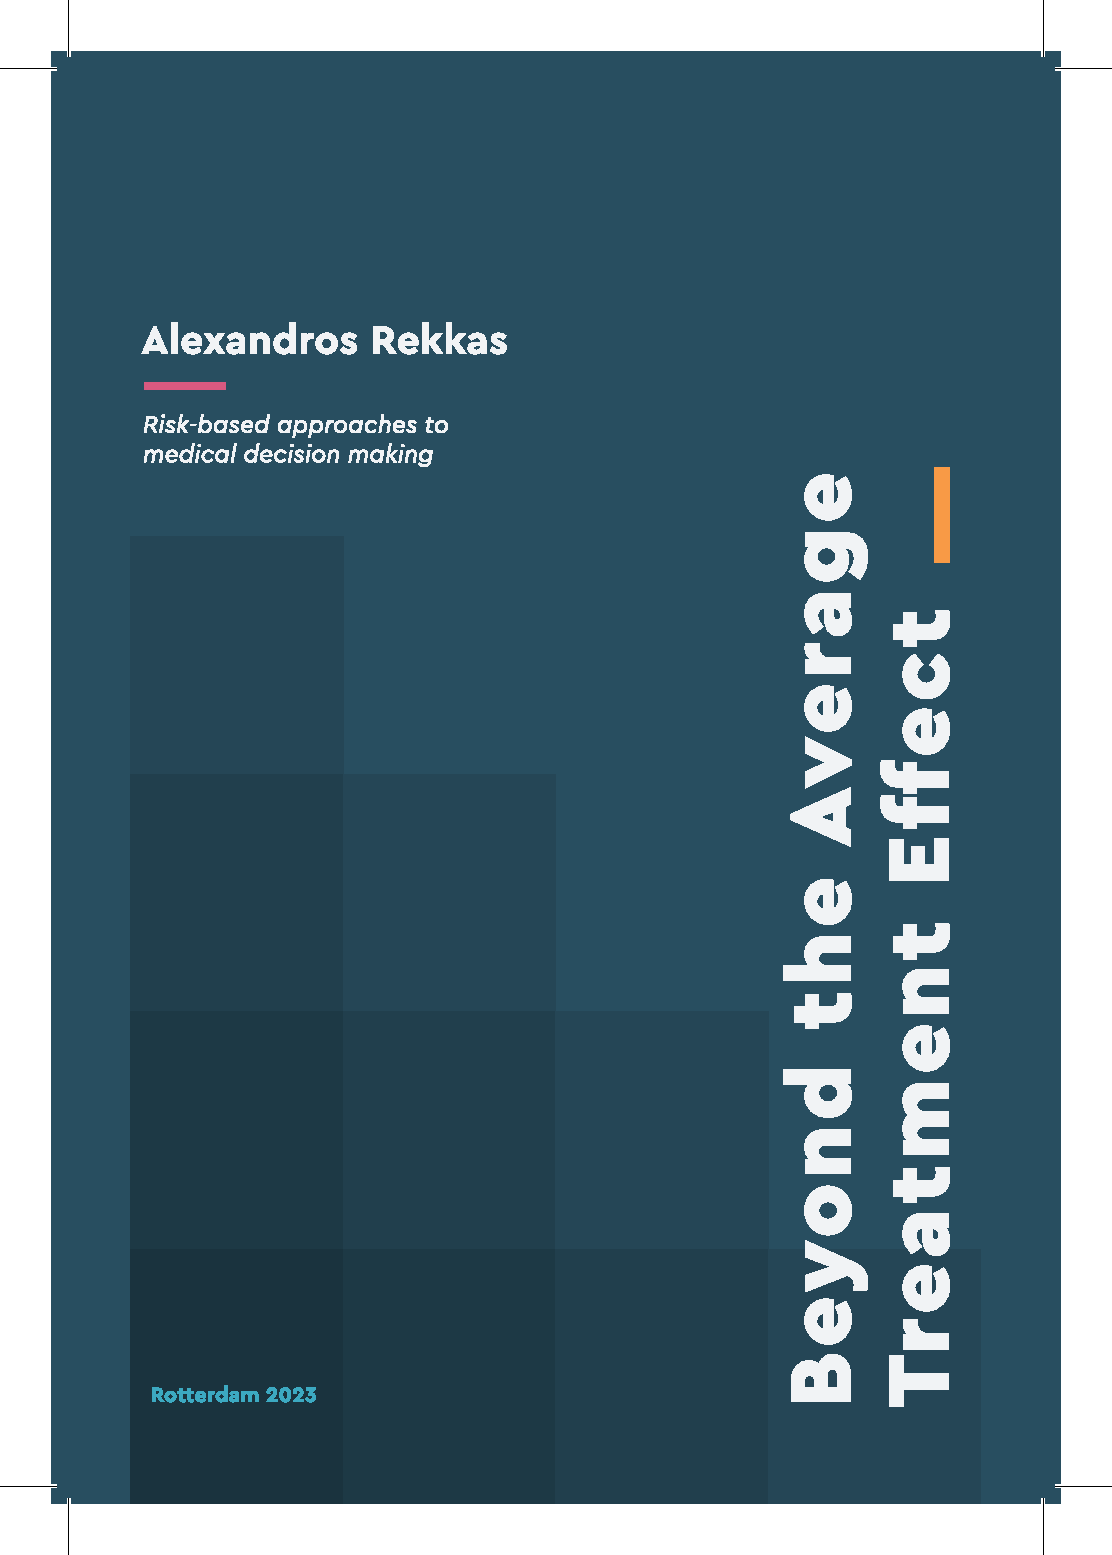
\includepdf{cover.pdf}


\clearpage\null\pagestyle{empty}
\newpage


% \thispagestyle{empty}
\pagestyle{empty}

\def\drop{.1\textheight}

\vspace*{6cm}
\begin{center}
\Large \textbf{\textsc{Beyond the Average Treatment Effect}}\par
\Large Risk-based approaches to medical decision making \par

\vspace*{1.8cm}

\Large Alexandros Rekkas

\end{center}

\clearpage

\thispagestyle{empty}
\vspace*{12cm}

\begingroup % to change formatting only temporarily
\small
\setlength{\parskip}{\baselineskip} % add space between paragraphs
\setlength\parindent{0pt} % no indents
Cover design: Anastassios Gkouvas \\
Printed by: Flyersonline | www.flyersonline.nl\\
\\
\begin{flushleft}
\textcopyright\ 2023 Alexandros Rekkas \\
All rights reserved. No part of this publication may be reproduced, distributed,
stored in a retrieval system, or transmitted in any form by any means, electronic,
mechanical, photocopying, recording or otherwise without the permission of the
author, or, when applicable, of the publishers of the scientific papers.
\end{flushleft}

\endgroup

\newpage
\thispagestyle{empty}

\begin{center}
\textbf{\textsc{Beyond the Average Treatment Effect}}\par
Risk-based approaches to medical decision making \par

\vspace*{0.6cm}

\textbf{\textsc{Voorbij het gemiddelde behandeleffect}}\par
Op risico gebaseerde benaderingen van medische besluitvorming \par

\vspace*{1cm}

\textbf{Proefschrift} \par

\vspace*{1cm}

ter verkrijging van de graad van doctor aan de\par
Erasmus Universiteit Rotterdam \par
op gezag van de \par
rector magnificus \par

\vspace*{0.8cm}

Prof.dr. A.L. Bredenoord\par

\vspace*{0.8cm}

en volgens besluit van het College voor Promoties. \par
De openbare verdediging zal plaatsvinden op  \par

\vspace*{0.4cm}

donderdag 2 November 2023 om 15.30 uur \par

\vspace*{0.4cm}

door \par

\vspace*{0.4cm}

Alexandros Rekkas \par

\vspace*{0.4cm}

geboren te Thessaloniki, Griekenland.

\end{center}


\begin{figure}[b]
\begin{subfigure}[][][b]{0.4\textwidth}
\includegraphics[width=1.2\linewidth]{figures/left.png}
\end{subfigure}\hspace{27mm}
\begin{subfigure}[][40pt][c]{0.6\textwidth}
\includegraphics[width=0.9\linewidth, height=2.4cm]{figures/right.png}
\end{subfigure}
\end{figure}

\newpage

\textbf{Promotiecommissie:}\par
\vspace*{0.8cm}

\begin{tabular}{l@{}l}
\textbf{Promotoren:} \mbox{} & Prof.dr.ir. P.R. Rijnbeek\\
                             & Prof.dr. E.W. Steyerberg \\
                             & \\
\textbf{Overige leden:} \mbox{} & Prof.dr. H.F. Lingsma \\
                                & Prof.dr. D. Rizopoulos \\
                                & Prof.dr. S. le Cessie \\
                                & \\
\textbf{Copromotor:} \mbox{} & Dr.ir. D. van Klaveren \\
\end{tabular}

\newpage
\addtocontents{toc}{\protect\thispagestyle{empty}}
\tableofcontents
\clearpage

